\section{Calcul bayésien avec OpenBUGS et JAGS}\label{annexe:openbugs-jags}

\subsection{Contexte de développement}

WinBUGS et son successeur OpenBUGS font partie du projet BUGS ({\it Bayesian inference Using Gibbs Sampler}) qui vise à rendre simple la pratique des méthodes MCMC aux statisticiens. Il a été développé par l'université de Cambridge. {\bf Seul OpenBUGS est actuellement maintenu}. \\

WinBUGS et OpenBUGS peuvent être utilisé de différentes manières :
\begin{itemize}
\item Via une interface « clique-bouton » qui permet de contrôler l'analyse,
\item En utilisant des modèles définis par des interfaces graphiques, appelés \texttt{DoddleBUGS},
\item Via d'autres logiciels tels que \texttt{R} (en particulier via le package \texttt{R2WinBUGS}).
\end{itemize}
WinBUGS et OpenBUGS sont des logiciels libres et gratuits, Cependant, afin d'accéder à la version non restreinte de WinBUGS, il est nécessaire d'obtenir la clé d'utilisation. Le site internet pour WinBUGS et OpenBUGS, {\bf The BUGS Project} présente les deux logiciels et fournit de la documentation. Le site spécialisé pour OpenBUGS est \url{http://www.openbugs.net/} \\

JAGS est une version "rapide" de BUGS développée par Martyn Plummer. Il repose sur le même language, à quelques différences subtiles près. Il a la particularité de ne pas présenter d'interface graphique pour la gestion des cha\^ines (mais il peut aussi être appelé par \texttt{R}). Traditionnellement, il possède moins de distributions de probabilité que sous OpenBUGS. 

\paragraph{D'autres outils logiciels.} Régulièrement, d'autres outils logiciels sont élaborés permettant de s'attaquer à des modèles à état latents, ou/et de grande dimension, mettant en oeuvre des MCMC accélérées... Citons le package Python \texttt{ELFI}\footnote{\url{https://elfi.readthedocs.io/en/latest/usage/tutorial.html}}, le langage \texttt{STAN} ou encore le langage \texttt{Birch}\footnote{\url{https://birch-lang.org/talks/automated-learning-slides.pdf}}. 

\subsection{Un exemple ``fil rouge" : le modèle bêta-binomial}

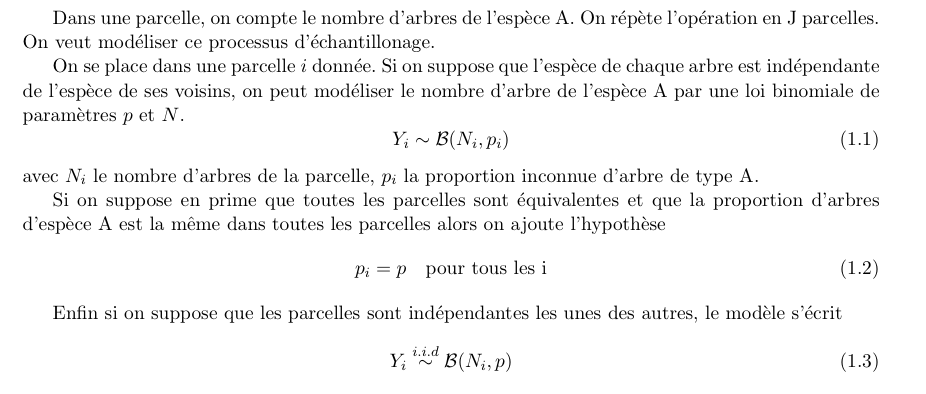
\includegraphics[scale=0.5]{figures/openbugsjags/betabin1.png} \\

\begin{center}
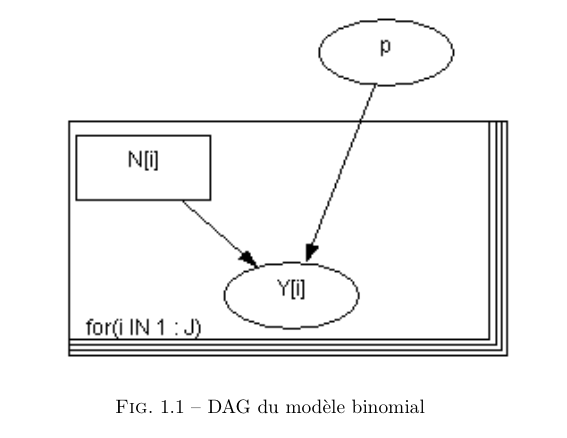
\includegraphics[scale=0.5]{figures/openbugsjags/beta-bin2.png} \\
\end{center}


\includegraphics[scale=0.5]{figures/openbugsjags/beta-bin3.png} \\

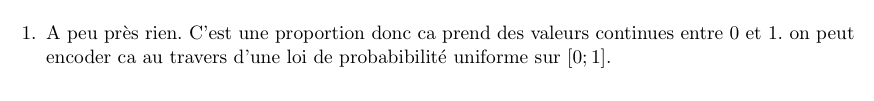
\includegraphics[scale=0.5]{figures/openbugsjags/beta-bin4.png} \\
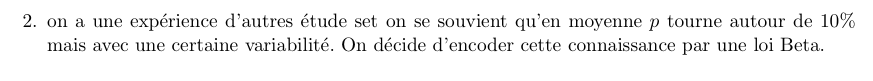
\includegraphics[scale=0.5]{figures/openbugsjags/beta-bin5.png} \\
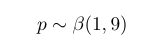
\includegraphics[scale=0.5]{figures/openbugsjags/beta-bin6.png} \\
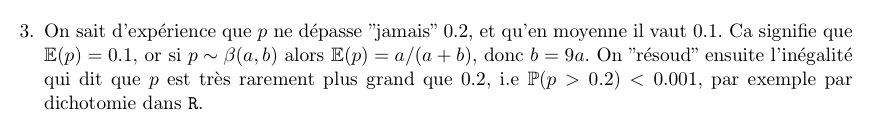
\includegraphics[scale=0.5]{figures/openbugsjags/beta-bin7.png} \\

On peut mener un calcul {\it a posteriori} par conjugaison. Avec 

 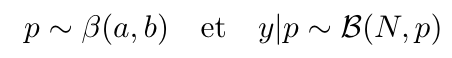
\includegraphics[scale=0.3]{figures/openbugsjags/beta-bin81.png} alors \\
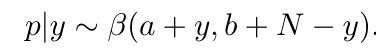
\includegraphics[scale=0.3]{figures/openbugsjags/beta-bin82.png} \\


\subsection{Fonctionnement résumé d'OpenBUGS}

\texttt{
\begin{enumerate}
\item Ouverture de la fenêtre OpenBUGS
\item Création d'un fichier "modele.txt" contenant l'écriture formelle de la \emph{vraisemblance} et de \emph{la distribution {\it a priori}}
\begin{itemize}
\item \scriptsize nécessité d'utiliser une boucle sur les données pour la vraisemblance
\item \scriptsize langage BUGS différent de R (mais plutôt compréhensible)
\end{itemize}
\item Création d'un fichier "data.txt" avec des données entrées en vectoriel (possibilité de tableaux)
\begin{itemize}
\item \scriptsize les "données" regroupent aussi les constantes du problème : taille des données $n$, etc. 
\end{itemize}
\item \'Eventuellement création d'un fichier d'initialisation pour les paramètres (cha\^ines MCMC)
\end{enumerate}
}

\vspace{1cm}

Testons ici l'implémentation du cas d'étude bêta-binomial. Ouvrons un fichier \texttt{model-beta-binomial.txt} (à ouvrir comme "Text") :

\begin{center} 
\fbox{ 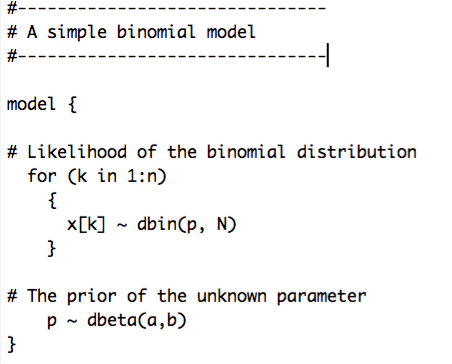
\includegraphics[scale=0.4]{figures/openbugsjags/beta-bin9.png}}
\end{center} 
\begin{enumerate}
    \item \emph{\bf Vérification du modèle} via \texttt{"Model/Model Specification"} puis \texttt{"Check Model"} 
    \begin{itemize}
        \item $\Rightarrow$ \emph{model is syntactically correct}
    \end{itemize}
    \item \emph{\bf  Enregistrement des données} via :
\begin{enumerate}
\item sélection du fichier \texttt{data-beta-binomial.txt}
\begin{center} 
 \fbox{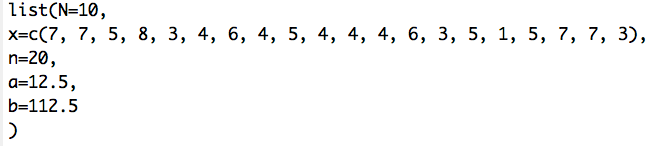
\includegraphics[scale=0.4]{figures/openbugsjags/beta-bin10.png}} 
 \end{center} 
 \item \texttt{"Load data"}
\end{enumerate}
\begin{itemize}
        \item $\Rightarrow$ \emph{data loaded}
    \end{itemize}
\item \emph{\bf Sélection du nombre de chaînes MCMC puis compilation du modèle} via \texttt{"compile"}
\begin{itemize}
        \item $\Rightarrow$ \emph{model compiled}
    \end{itemize}
    \item \emph{\bf Initialisation des chaînes MCMC} : 2 fa\c cons possibles
\begin{enumerate}
\item Sélection dans le fichier \texttt{init-beta-binomial.txt} puis \texttt{"load inits"}, chaîne par chaîne
\item Génération automatique via \texttt{"gen inits"} pour toutes les chaînes 
\begin{itemize}
        \item $\Rightarrow$ \emph{model initialized}
    \end{itemize}
\end{enumerate}
\item \emph{\bf Ouverture de la fenêtre de monitoring des chaînes} via \texttt{"Inference/Sample Monitor Tool"}
\begin{itemize}
\item \'Ecrire \texttt{"p"} dans la fenêtre \texttt{"node"}, valider avec \texttt{"set"}
\end{itemize}
\item  \emph{\bf Ouverture de la fenêtre de lancement des chaînes} via \texttt{"Model/Update"}
\begin{itemize}
\item cliquer sur \texttt{"update"} pour lancer une première fois les chaînes  
\item  $\Rightarrow$ \emph{model is updating}
\end{itemize}
\item \emph{\bf  Monitorer les chaînes} via la fenêtre consacrée :
\begin{itemize}
\item Aller chercher \texttt{"p"} dans la fenêtre \texttt{"node"}, puis cliquer sur :
\item \scriptsize  \texttt{"trace"} pour tracer l'évolution des chaînes associées à $p$
\item \scriptsize \texttt{"trace"} pour tracer la densité {\it a posteriori} courante (approximative)
\item \scriptsize \texttt{"coda"} pour récupérer les chaînes
\item \scriptsize \texttt{"stats"} pour obtenir un résumé statistique de la loi {\it a posteriori} courante 
\item  \scriptsize  etc.
\end{itemize}
\end{enumerate}


\subsection{Quelques détails supplémentaires concernant OpenBUGS}

\paragraph{Menu ``Infererence".}
\begin{enumerate}
\item \emph{\bf Sous-menu \texttt{"Correlation"}} 
\begin{itemize}
\item \texttt{"Correlation Tool"} 
\begin{itemize}
\item \scriptsize  \texttt{scatter} $\Rightarrow$ trace un "scatterplot" entre 2 dimensions
\item  \scriptsize  \texttt{matrix} $\Rightarrow$ dessine la matrice de corrélation (par niveaux de gris)
\item  \scriptsize  \texttt{print} $\Rightarrow$ calcule le coefficient de corrélation linéaire 
\end{itemize}
\end{itemize}
\item \emph{\bf Sous-menu \texttt{"Compare"}} 
\begin{itemize}
\item \texttt{"Comparison Tool"} 
\begin{itemize}
\item \scriptsize  \texttt{boxplot} $\Rightarrow$ trace une "boîte à moustaches" d'une dimension sélectionnée
%\item  \scriptsize  \texttt{density strips} $\Rightarrow$ dessine la matrice de corrélation (par niveaux de gris)
%\item  \scriptsize  \texttt{print} $\Rightarrow$ calcule le coefficient de corrélation linéaire 
\end{itemize}
\end{itemize}
\end{enumerate}

\paragraph{Menu ``Model".}
\begin{itemize}
\item Commande  \emph{\texttt{"latex"}} : fournit le code latex du fichier sélectionné (utile pour le fichier de modèle !)
\end{itemize}

\subsection{Liste des distributions de probabilités disponibles}

\begin{tabular}{ll}
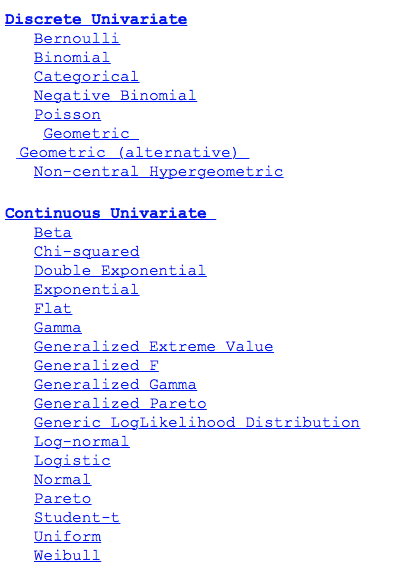
\includegraphics[scale=0.4]{figures/openbugsjags/tab1.png} & 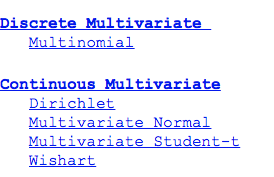
\includegraphics[scale=0.4]{figures/openbugsjags/tab2.png}
\end{tabular}

\subsection{Noeuds logiques et indexation}

 Les noeuds logiques sont définis par une flèche et sont {\bf toujours indexés} : \\
 
 \begin{center} 
 \fbox{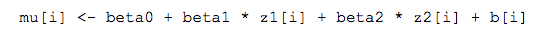
\includegraphics[scale=0.4]{figures/openbugsjags/var1.png}} 
 \end{center} 

On peut utiliser une fonction de lien (log, logit, probit) : \\

 \begin{center} 
 \fbox{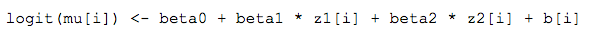
\includegraphics[scale=0.4]{figures/openbugsjags/var2.png}} 
 \end{center} 
 
 On peut définir des tableaux : \\
 
  \begin{center} 
 \fbox{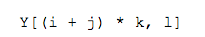
\includegraphics[scale=0.4]{figures/openbugsjags/var3.png}} 
 \end{center} 
 
Par ailleurs, toute variable (noeud logique ou stochastique \textasciitilde ) ne peut apparaître qu'une fois dans la partie gauche d'une expression (sauf dans le cas d'une transformation de données) du type :
 
   \begin{center} 
 \fbox{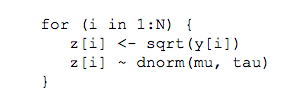
\includegraphics[scale=0.4]{figures/openbugsjags/var4.png}} 
 \end{center} 
 
 Enfin, on peut créer des noeuds multiparités : soient $\mu$ et $\tau$ deux vecteurs de taille $K$. On peut alors définir la boucle suivante :
 
    \begin{center} 
 \fbox{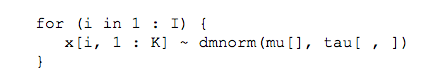
\includegraphics[scale=0.4]{figures/openbugsjags/var5.png}} 
 \end{center} 

L'aide sur les fonctions utiles est disponible ici : \url{http://www.openbugs.net/Manuals/ModelSpecification.html} \\

\subsection{Pièges à éviter}

Deux pièges peuvent fréquemment survenir :
\begin{itemize}
    \item {\bf Se tromper de paramétrisation}. Il faut toujours aller vérifier de quelle fa\c con les distributions de probabilité sont définies ! C'est piégeant en particulier pour les lois normale et log-normale :
        \begin{center} 
 \fbox{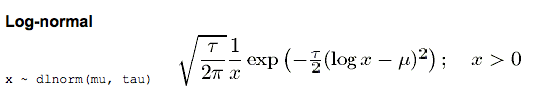
\includegraphics[scale=0.4]{figures/openbugsjags/tab3.png} } 
  \fbox{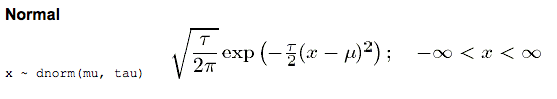
\includegraphics[scale=0.4]{figures/openbugsjags/tab4.png} } 
 \end{center} 
    
    \item {\bf Confondre censure et troncature}. La \emph{censure} est possible en utilisant la notation suivante :
     \begin{center} 
 \fbox{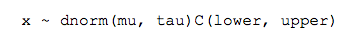
\includegraphics[scale=0.4]{figures/openbugsjags/cen1.png} } 
 \end{center} 
    Il s'agit d'une censure par intervalle. On laisse un blanc à gauche ({\it resp.} à droite) si la donnée est censurante à droite ({\it resp.} à gauche). La \emph{troncation} est possible en utilisant la notation suivante :
       \begin{center} 
 \fbox{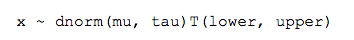
\includegraphics[scale=0.4]{figures/openbugsjags/cen2.png} } 
 \end{center}
\end{itemize}

Notons enfin que Les priors impropres (non intégrables) ne sont pas utilisables en BUGS. Il faut les approcher avec des distributions propres mais de variance très large (ce qui est dangereux hélas). Une "règle du pouce" pour les paramètres de variance inverse est la suivante : 
 \begin{eqnarray*}
\tau &  \sim & \text{dgamma(0.001, 0.001)}
 \end{eqnarray*} 
 mais l'usage d'OpenBUGS, JAGS, etc. nécessite donc de toujours mener des études de sensibilité {\it a posteriori}. Enfin, l'implémentation d'une nouvelle distribution est possible, mais il faut utiliser des subterfuges, typiquement par une transformation de variables (ex : Box-M\"uller pour simuler des gaussiennes).

\subsection{Utilisation d'OpenBUGS avec \texttt{R}}

Plusieurs packages sont disponibles pour appeler un code OpenBUGS depuis \texttt{R} : BRugs, R2WinBUGS et R2OpenBUGS. Nous recommandons l'usage du dernier, qui nécessite d'installer également le package CODA (gestion des MCMC) :
\begin{enumerate}
    \item  Installer le package R2OpenBUGS {(nécessite CODA)}.
    \item Le charger dans un programme \texttt{R} avec \texttt{library(R2OpenBUGS)}.
    \item Définir le répertoire où se trouve les fichiers BUGS comme répertoire de travail courant, par exemple :
    \begin{center} 
 \fbox{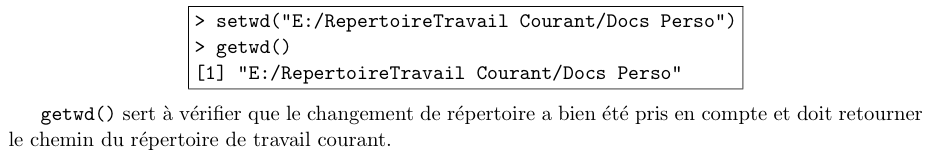
\includegraphics[scale=0.4]{figures/openbugsjags/esso.png} } 
 \end{center}
 \item Spécification du modèle :
   \begin{center} 
 \fbox{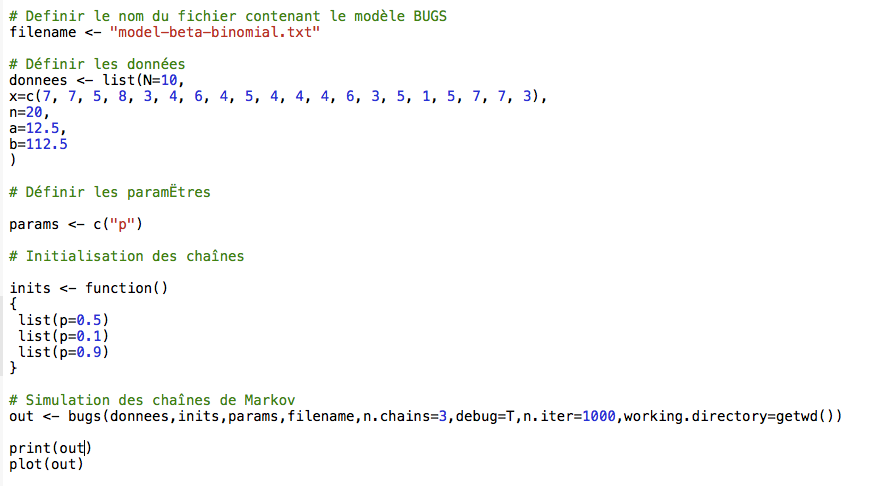
\includegraphics[scale=0.4]{figures/openbugsjags/esso2.png} } 
 \end{center}
  \item Obtention des résultats : avec \texttt{debug=T}, fermer la fenêtre OpenBUGS qui s'est ouverte pour achever le traitement numérique. Le répertoire courant doit se présenter ainsi : 
   \begin{center} 
 \fbox{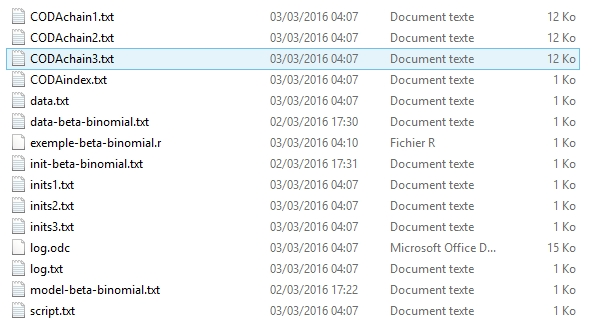
\includegraphics[scale=0.4]{figures/openbugsjags/res.jpeg} } 
 \end{center}
\end{enumerate}

\subsection{Détails sur JAGS : exemple de script}

   \begin{center} 
 \fbox{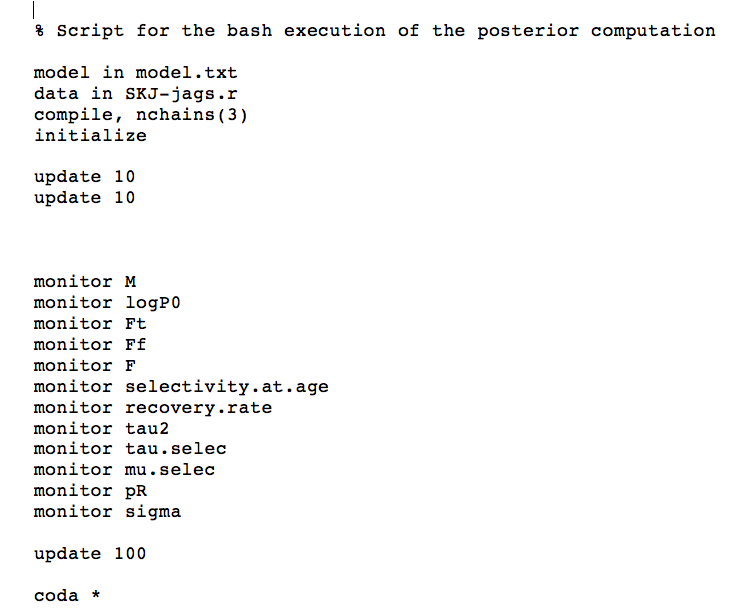
\includegraphics[scale=0.4]{figures/openbugsjags/res01.png} } 
 \end{center}

\subsection{D'autres outils (R/Python)}

\texttt{Nimble} est un outil permettant de lancer des tâches de calcul bayésien à partir de \texttt{R}. Pour \texttt{Python 3}, on pourra explorer et utiliser \texttt{Pymc}. 